\subsection{Estructura de Bandas}
\begin{frame}[t]
\frametitle{Introducci\'on}
\framesubtitle{Estructura de Bandas}
\vspace{-0.5cm}
\begin{tikzpicture}[remember picture, overlay]
\node<1->[anchor = north west, text width =0.7\textwidth, yshift = -0.75cm](txt) at (current page.north west) {
	\begin{tcolorbox}[enhanced,title =Estructura de Bandas,
	left=1mm,
	top=1mm,
	bottom=1mm,
	right=1mm,
	width =\textwidth,
	height=0.45\textheight,
	boxsep = 0cm,
	coltitle=blue,
	attach boxed title to top center={yshift=-2mm,yshifttext=-1mm},
	boxed title style={colframe=blue,
		colback=gc!90}]
	\begin{itemize}
	\item<1-> Dicta el comportamiento de los electrones dentro de un solido
	\item<2-> En un solido $\approx 10^{23}$ atomos\\$\rightarrow$\text{\color{red}problema complejo de muchos cuerpos}
	\item<3-> Hamiltoniano de un solido
	\item<4-> Gracias al Teorema de Bloch\\ $\rightarrow$ potencial periodico
	\item<5-> Ecuacion de Schr\"odinger en terminos de un el\'ectron. 
	\end{itemize}
	\end{tcolorbox}	
};

\node<1->[anchor=north east,xshift=-2cm,yshift=-1cm] at (current page.north east){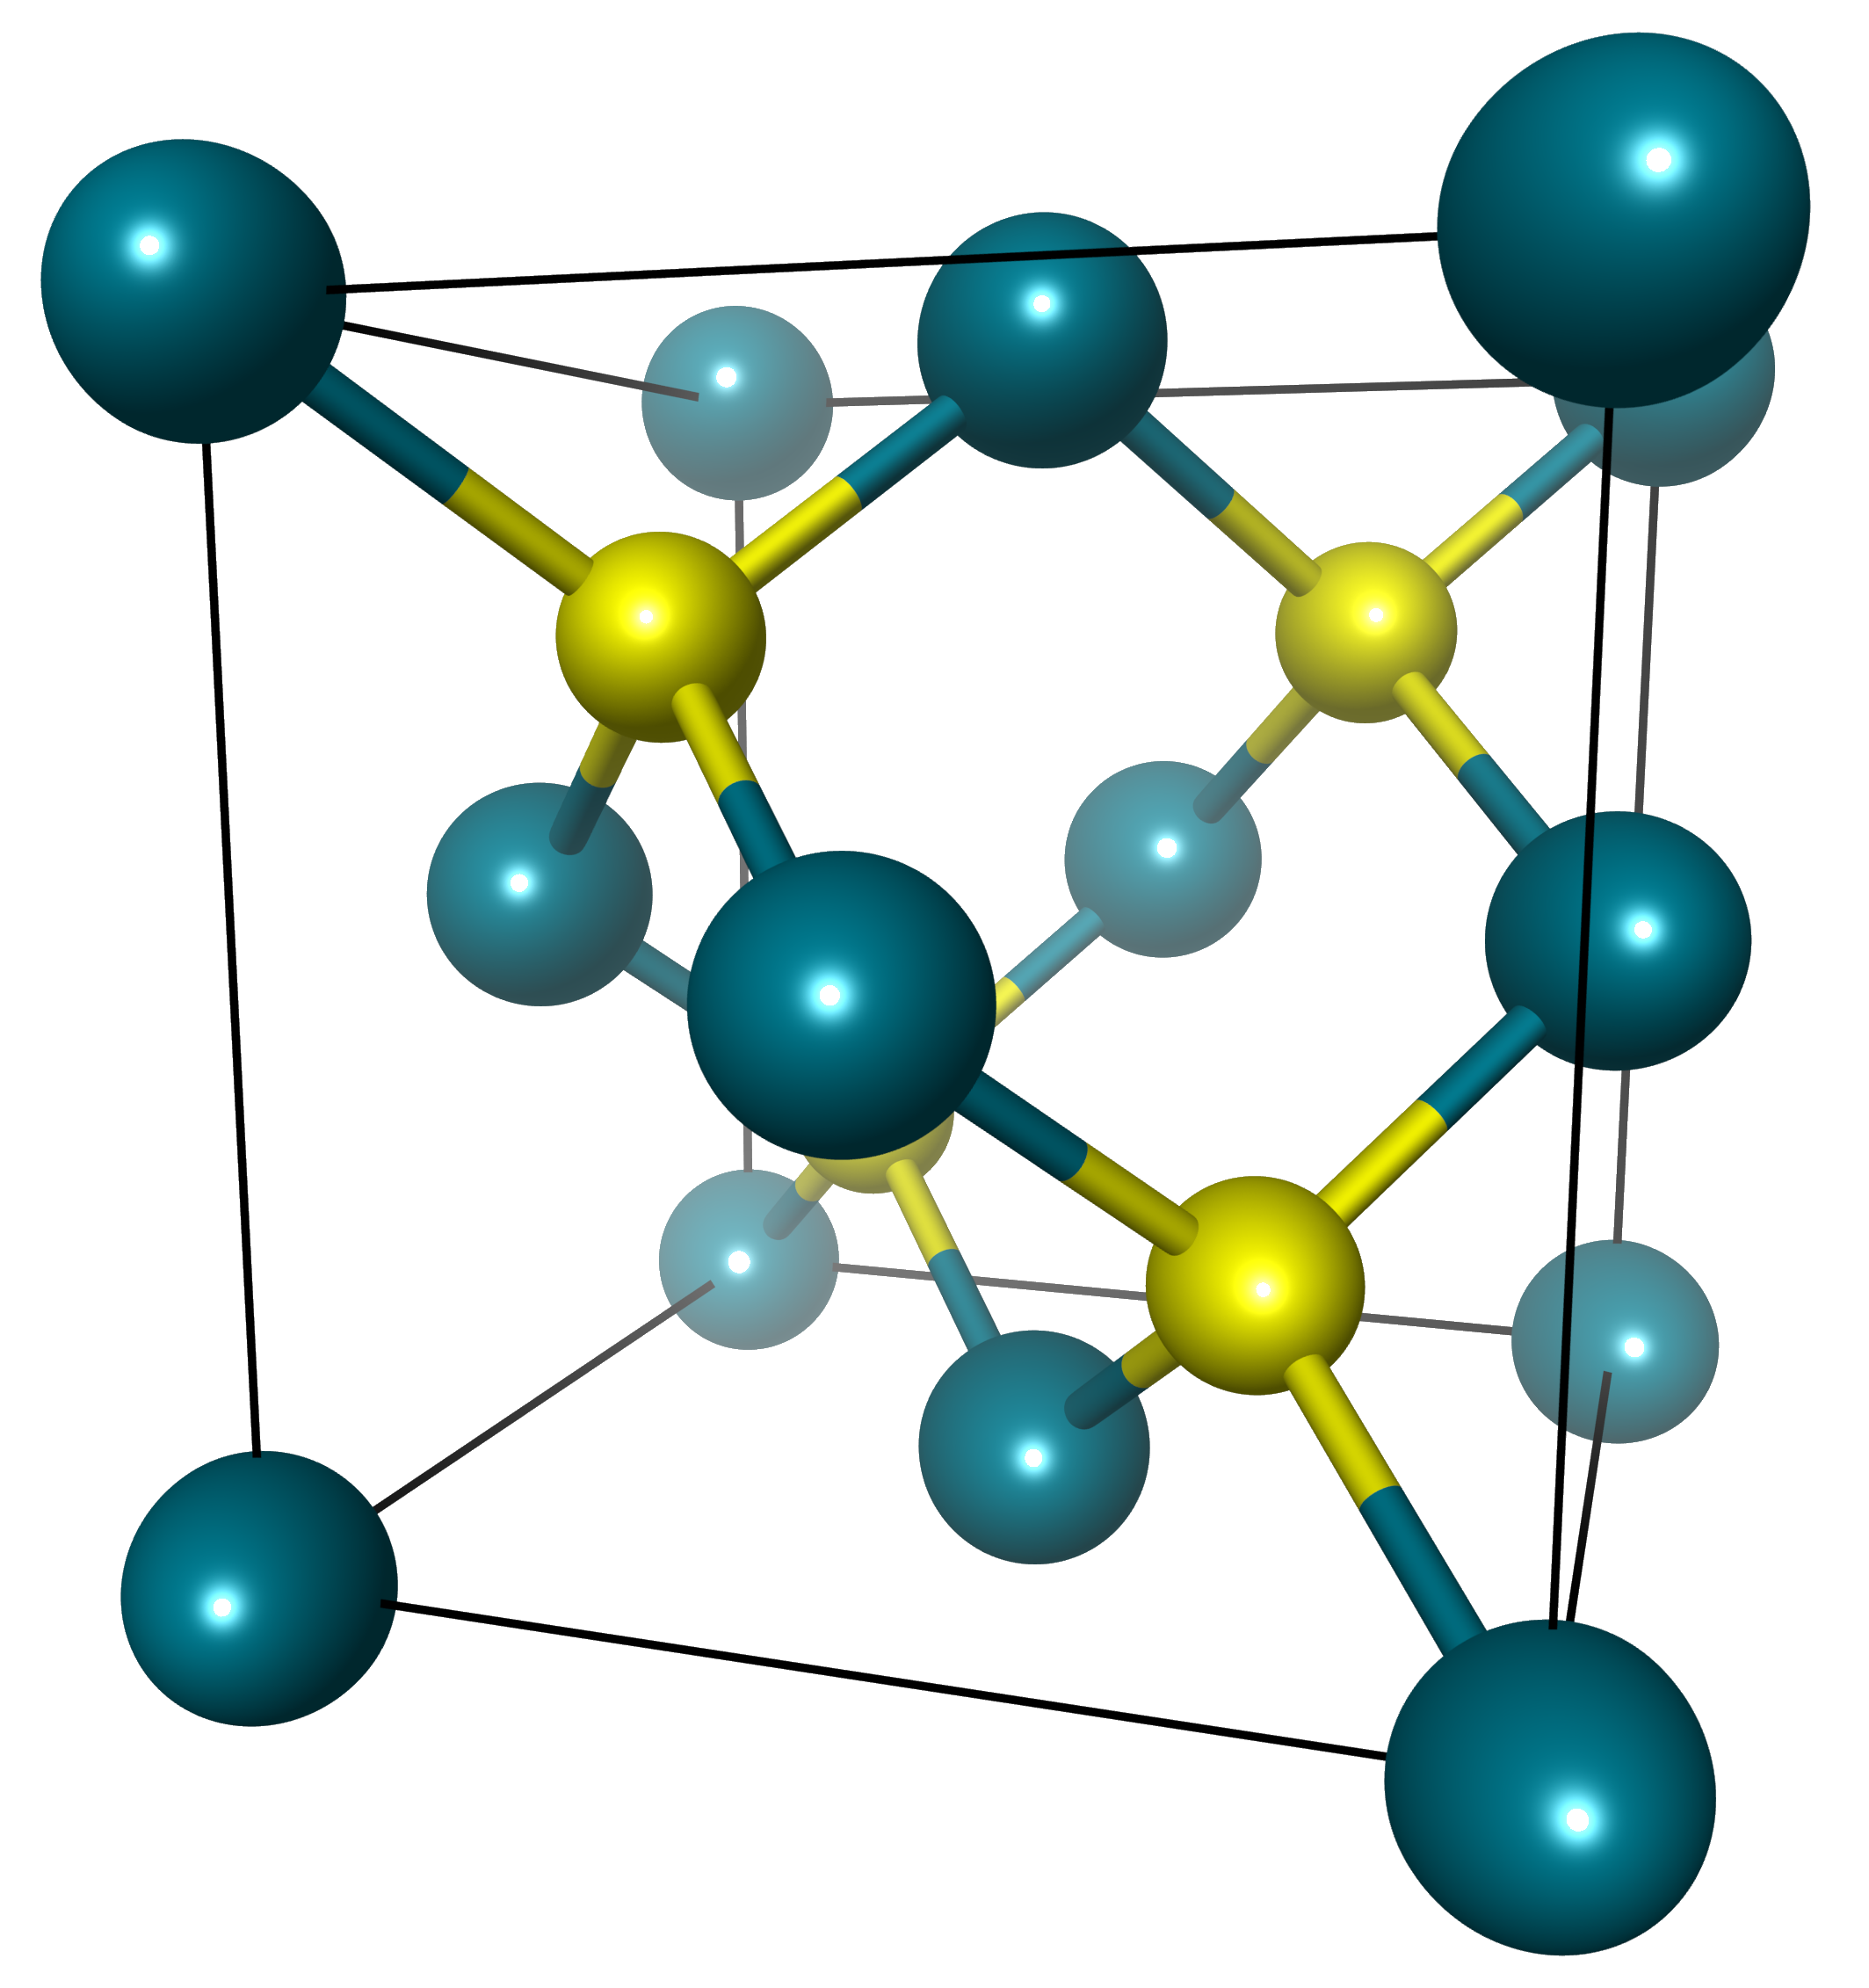
\includegraphics[width=0.35\textwidth]{../../../scripts/structures/GaAs-2}};

\node<3>[anchor=center,text width=\textwidth,font=\sffamily,xshift=-1cm,yshift=-2cm] at (current page.center){
\begin{equation*}
	\begin{split}
	H  =  &\dfrac{1}{2M}\sum\limits_{i=1}^{N_{n}} \bff{P}_{j}^{2} + \dfrac{1}{2m_{0}} \sum\limits_{j=1}^{N_{e}} \bff{p}_{j}^{2} + \dfrac{Z^{2}}{2} \sum\limits_{i,j=1,i\neq j}^{N_{n}} V_{c}\left(\bff{R}_{i}-\bff{R}_{j}\right)-Z\sum\limits_{i=1}^{N_{n}}\sum\limits_{j=1}^{N_{e}}V_{c}\left(\bff{r}_{j}-\bff{R}_{i}\right) \\
	& + \dfrac{1}{2} \sum\limits_{i,j=1,i\neq j}^{N_{e}} V_{c} \left(\bff{r}_{i}-\bff{r}_{j}\right)
	\end{split}
\end{equation*}
};

\node<4->[anchor=south west,opacity=0.5](i1) at (current page.south west){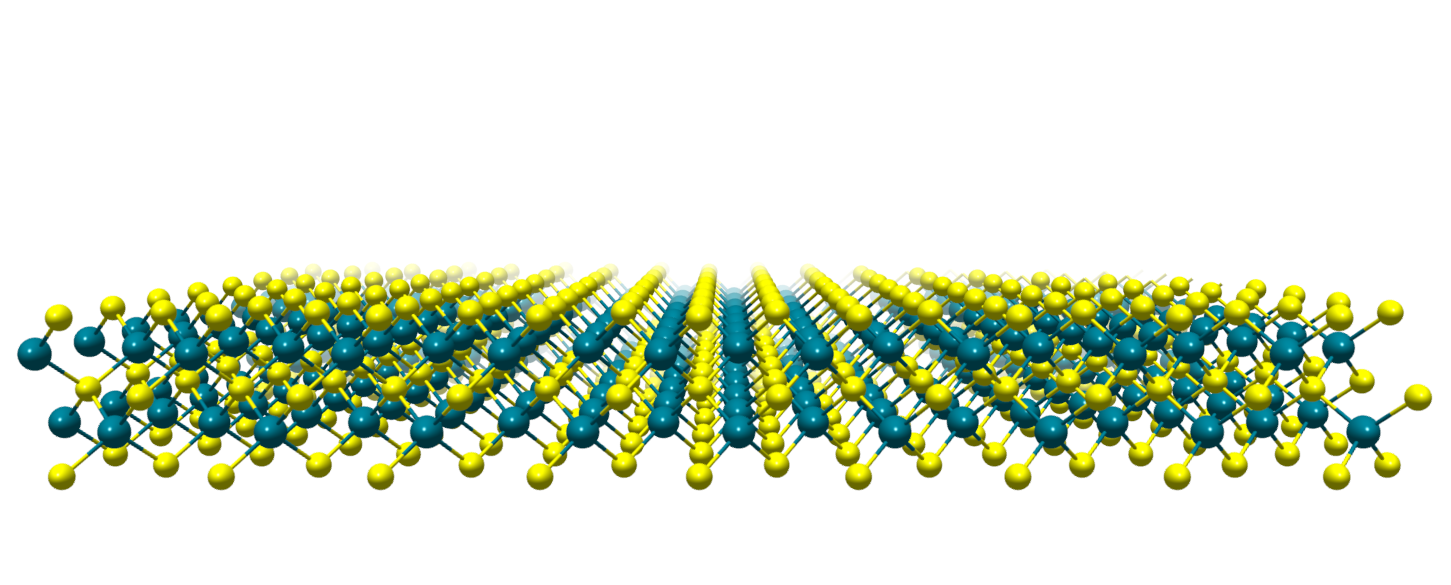
\includegraphics[width=\textwidth,trim = {0cm 0cm 0cm 2cm},clip]{beamer-figures/introduction/atom-line.png}};
\node<4->[anchor=center,yshift=0cm,inner sep=0mm,yshift=-0.5cm](bloch) at (i1.center){\animategraphics[autoplay,loop,width=\textwidth]{8}{beamer-figures/introduction/b1}{}{}};

\node<4->[anchor=south west,text width=\textwidth,scale=0.7] at (current page.south west) {Image credit: from \href{https://commons.wikimedia.org/wiki/File:Standing_wave.gif}{Wikimedia Commons}, public domain};
\node<5->[anchor=south west,yshift=-0.5cm,inner sep=0mm](schrodinger)at(bloch.north){$\left[-\dfrac{\hbar^2}{2m_{0}}\nabla^2 + U(\rv)\right]\psi (r)=\senergy\psi(\rv)$}; 


\end{tikzpicture}
\end{frame}


\begin{frame}[t]
	\frametitle{Introducci\'on}
	\framesubtitle{Bandas de Valencia y Conducci\'on para un semiconductor en Bulto}
	\vspace{-0.5cm}
	\begin{tikzpicture}[remember picture, overlay]
	\node<1-2>[anchor=north east,xshift=-2cm,yshift=-0.9cm] at (current page.north east){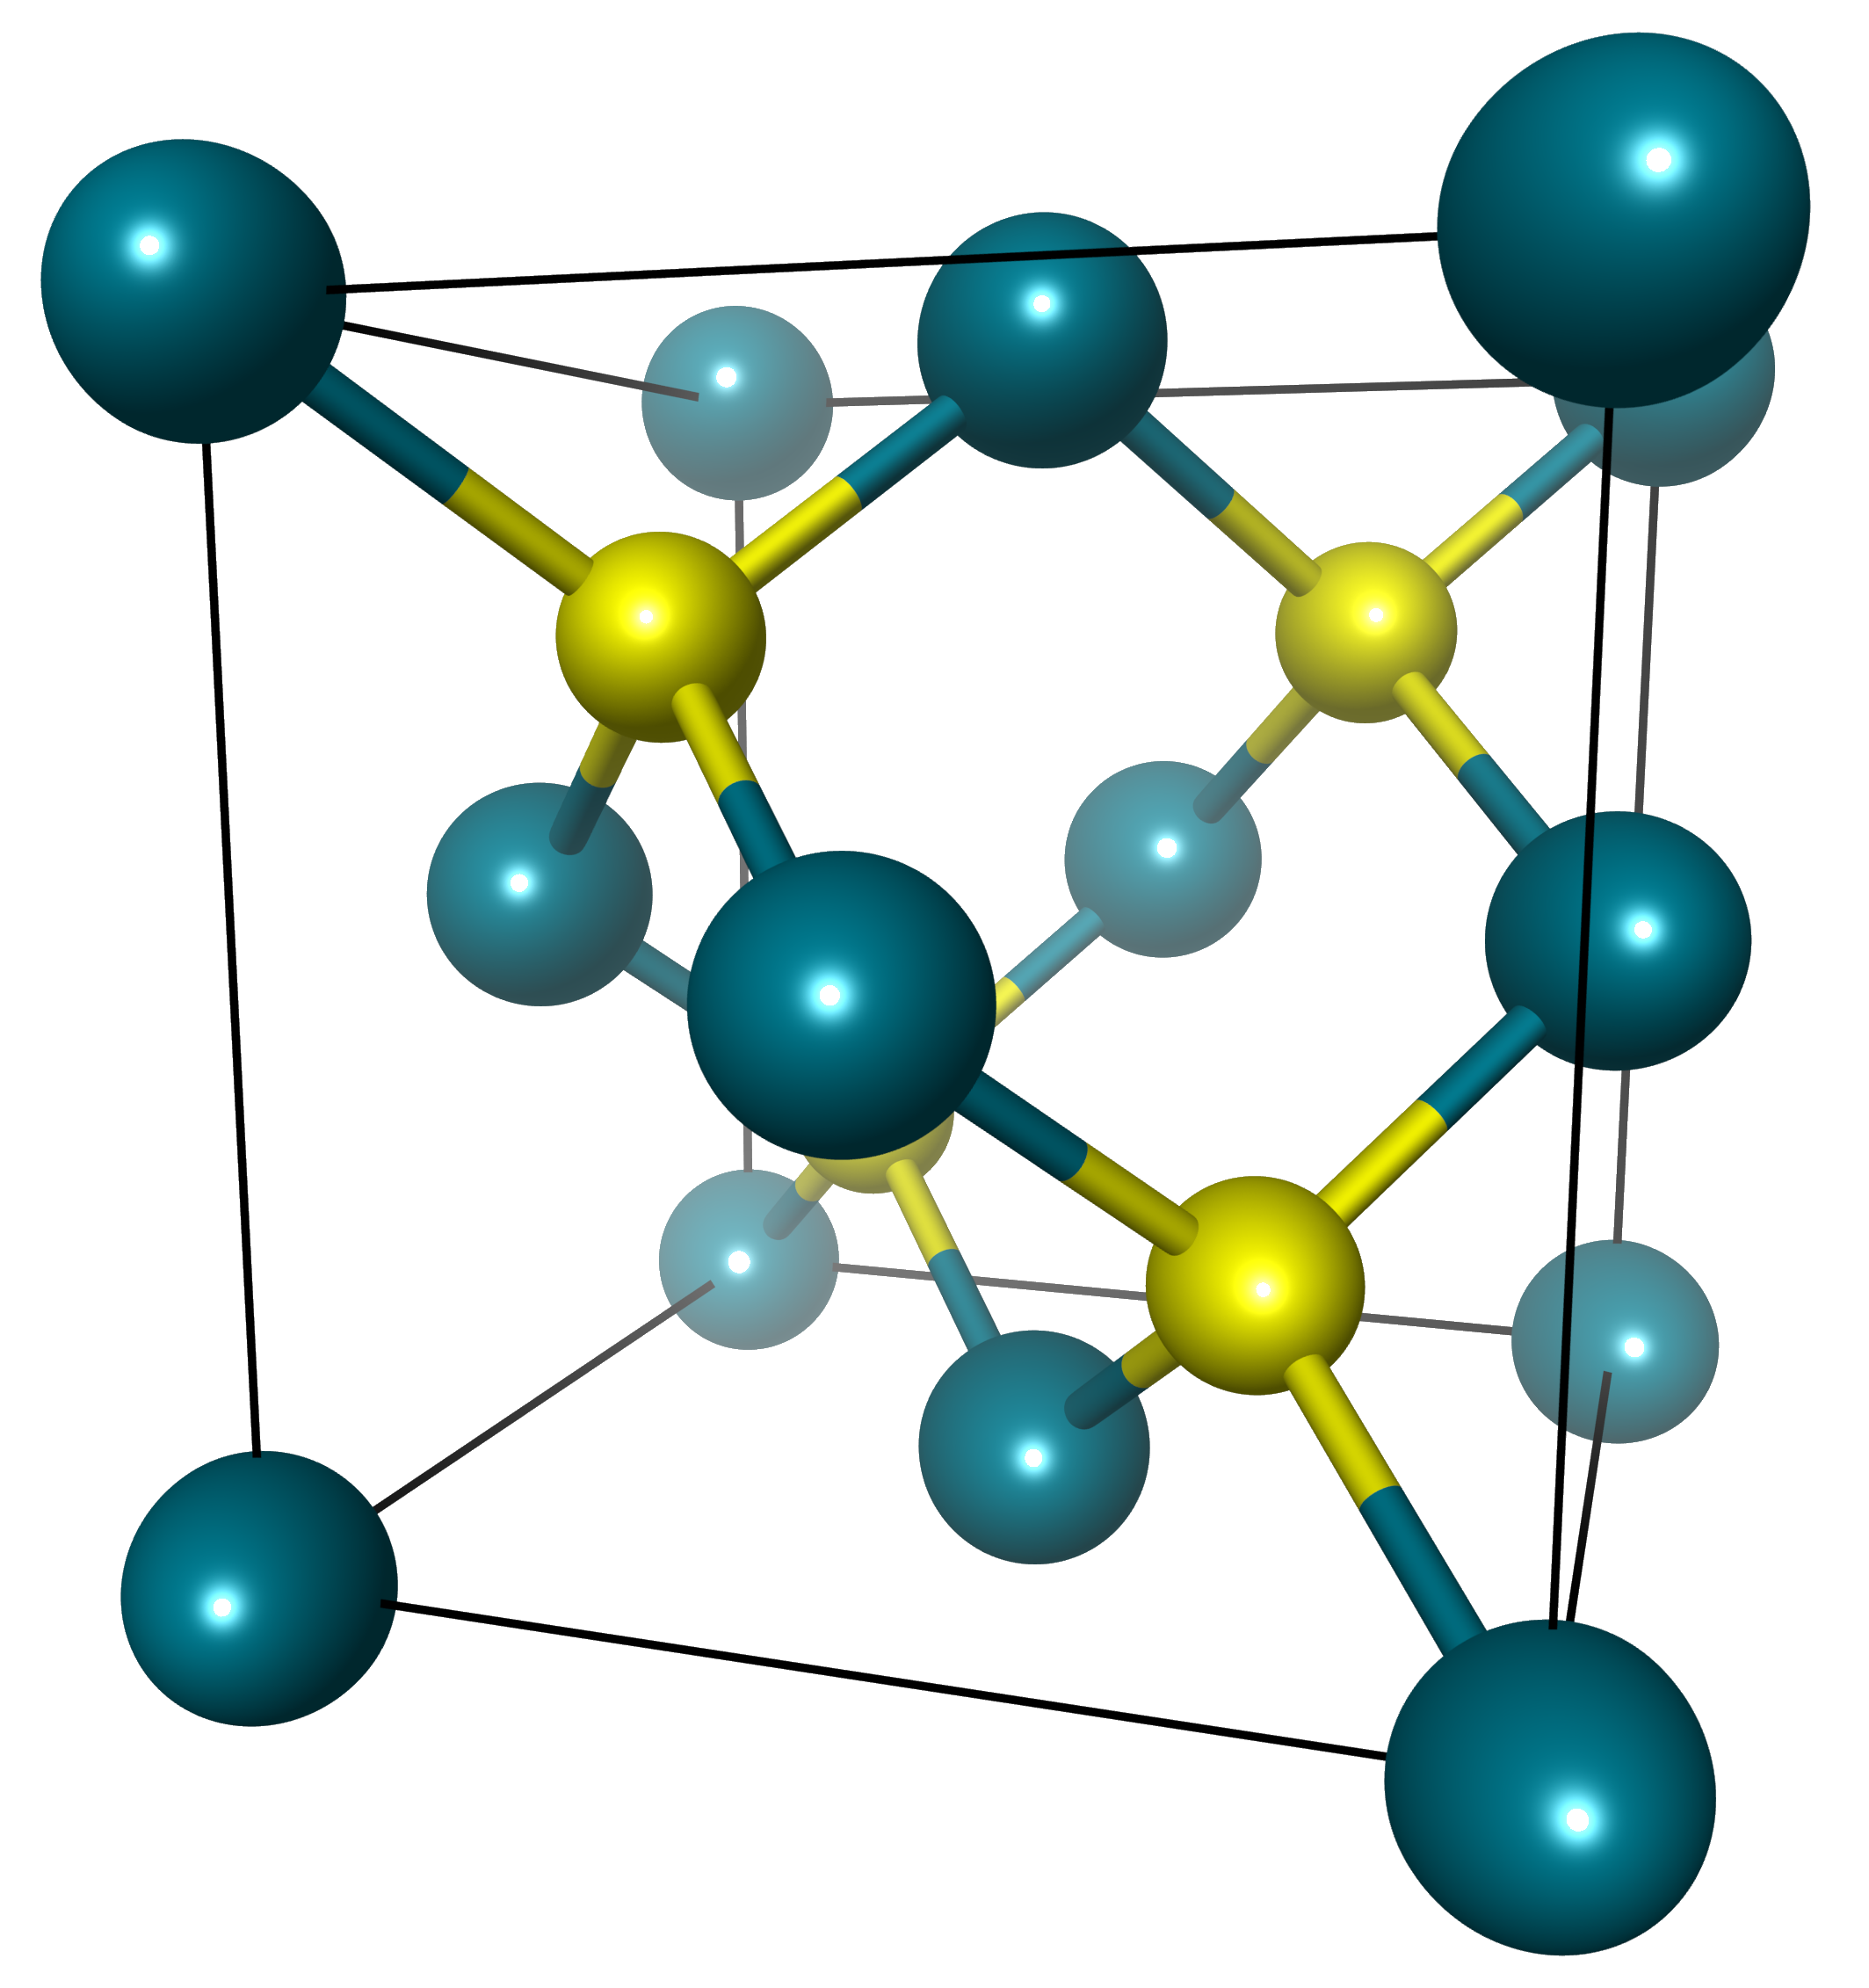
\includegraphics[width=0.35\textwidth]{../../../scripts/structures/GaAs-2}};
	\node<1-2>[anchor=north west,inner sep=0mm,yshift=-0.9cm](h) at (current page.north west){\animategraphics[autoplay,loop,width=0.3\textwidth]{1}{beamer-figures/introduction/build-ruco/H}{}{}};
\node<1-2>[anchor=north west,text width=0.2\textwidth,font=\sffamily,xshift=0cm,yshift=0.7cm,scale=2,blue](e1) at (h.south west){
\begin{equation*}
	\left(\tikzmarknode{a}{\mathcal{H}}-\varepsilon(\mathbf{k}\lambda)\ket{\mathbf{k\lambda}}\right)=0
\end{equation*}
};

\node<2>[anchor=north west,text width=2.2\textwidth,font=\sffamily,text=white,fill=black,yshift=1cm,scale=0.565] at (e1.south west){
$ \tikzmarknode{b}{\mathcal{H}}=
\begin{pmatrix}
E\left(s,a\right)&v\left(s,a\right)g_{0}&0&0&0&v\left(sa,pc\right)g_{1}&v\left(sa,pc\right)g_{2}&v\left(sa,pc\right)g_{3}&0&0\\
v\left(s,a\right)g_{0}^{*}&E\left(s,c\right)&-v\left(pa,sc\right)g_{1}^{*}&-v\left(pa,sc\right)g_{2}^{*}&-v\left(pa,sc\right)g_{3}^{*}&0&0&0&0&0\\
0&-v\left(pa,sc\right)g_{1}&E(p,a)&0&0&v\left(x,x\right)g_{0}&v\left(x,y\right)g_{3}&v\left(x,y\right)g_{2}&0&-v\left(pa,s^{*}\!c\right)g_{1}\\
0&-v\left(pa,sc\right)g_{2} &0&E\left(p,a\right)&0&v\left(x,y\right)g_{2}&v\left(x,y\right)g_{1} &v\left(x,y\right)g_{1} &0 &-v\left(pa,s^{*}\!c\right)g_{2}\\
0&-v\left(pa,sc\right)g_{3} &0&0&E\left(p,a\right) &v\left(x,y\right)g_{2} &v\left(x,y\right)g_{1} &v\left(x,x\right)g_{0} &0 &-v\left(pa,s^{*}\!c\right)g_{3}\\ 
v\left(sa,pc\right)g_{1}^{*}&0&v\left(x,x\right)g_{0}^{*}&v\left(x,y\right)g_{3}^{*} &v\left(x,x\right)g_{2}^{*} &E(p,c) &0 &0 &v\left(s^{*}\!a,pc\right)g_{1}^{*}&0  \\ 
v\left(sa,pc\right)g_{2}^{*}&0&v\left(x,y\right)g_{3}^{*}&v\left(x,x\right)g_{0}^{*}&v\left(x,y\right)g_{1}^{*} &0 &E(p,c) &0 &v\left(s^{*}\!a,pc\right)g_{2}^{*}&0  \\ 
v\left(sa,pc\right)g_{3}^{*}&0&v\left(x,y\right)g_{2}^{*}&v\left(x,y\right)g_{1}^{*}&v\left(x,x\right)g_{0}^{*} &0 &0 &E(p,c)&v\left(s^{*}\!a,pc\right)g_{3}^{*}&0 \\ 
0&0&0&0  &0 &v\left(s^{*}\!a,pc\right)g_{1}^{*} &v\left(s^{*}\!a,pc\right)g_{2}^{*} &v\left(s^{*}\!a,pc\right)g_{3}^{*} &E(s^{*}\!,a)&v(s^{*}\!.s^{*}\!)g_{0} \\ 
0&0&-v\left(pa,s^{*}\!c\right)g_{1}^{*}&-v\left(pa,s^{*}\!c\right)g_{2}^{*}  &-v\left(pa,s^{*}\!c\right)g_{3}^{*} &0 &0 &0 &v(s^{*}\!.s^{*}\!)g_{0}&E(s^{*}\!,c)  
\end{pmatrix}
$};

%==========> parte 2
\node<3->[anchor=north west,yshift=-9mm,inner sep=0mm](s) at (current page.north west){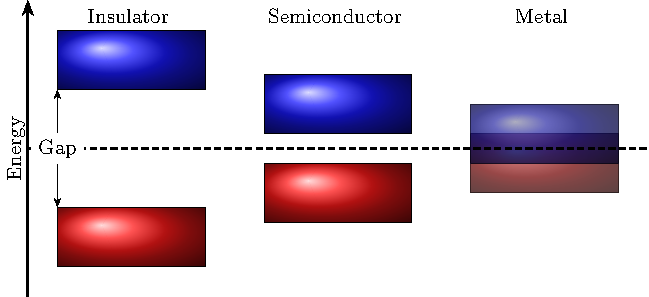
\includegraphics[width=0.7\textwidth]{../../figures/chapter-1/solid-sort/build/solid-sort}};
\node<3->[anchor=north east,xshift=-2cm,yshift=-0.9cm] at (current page.north east){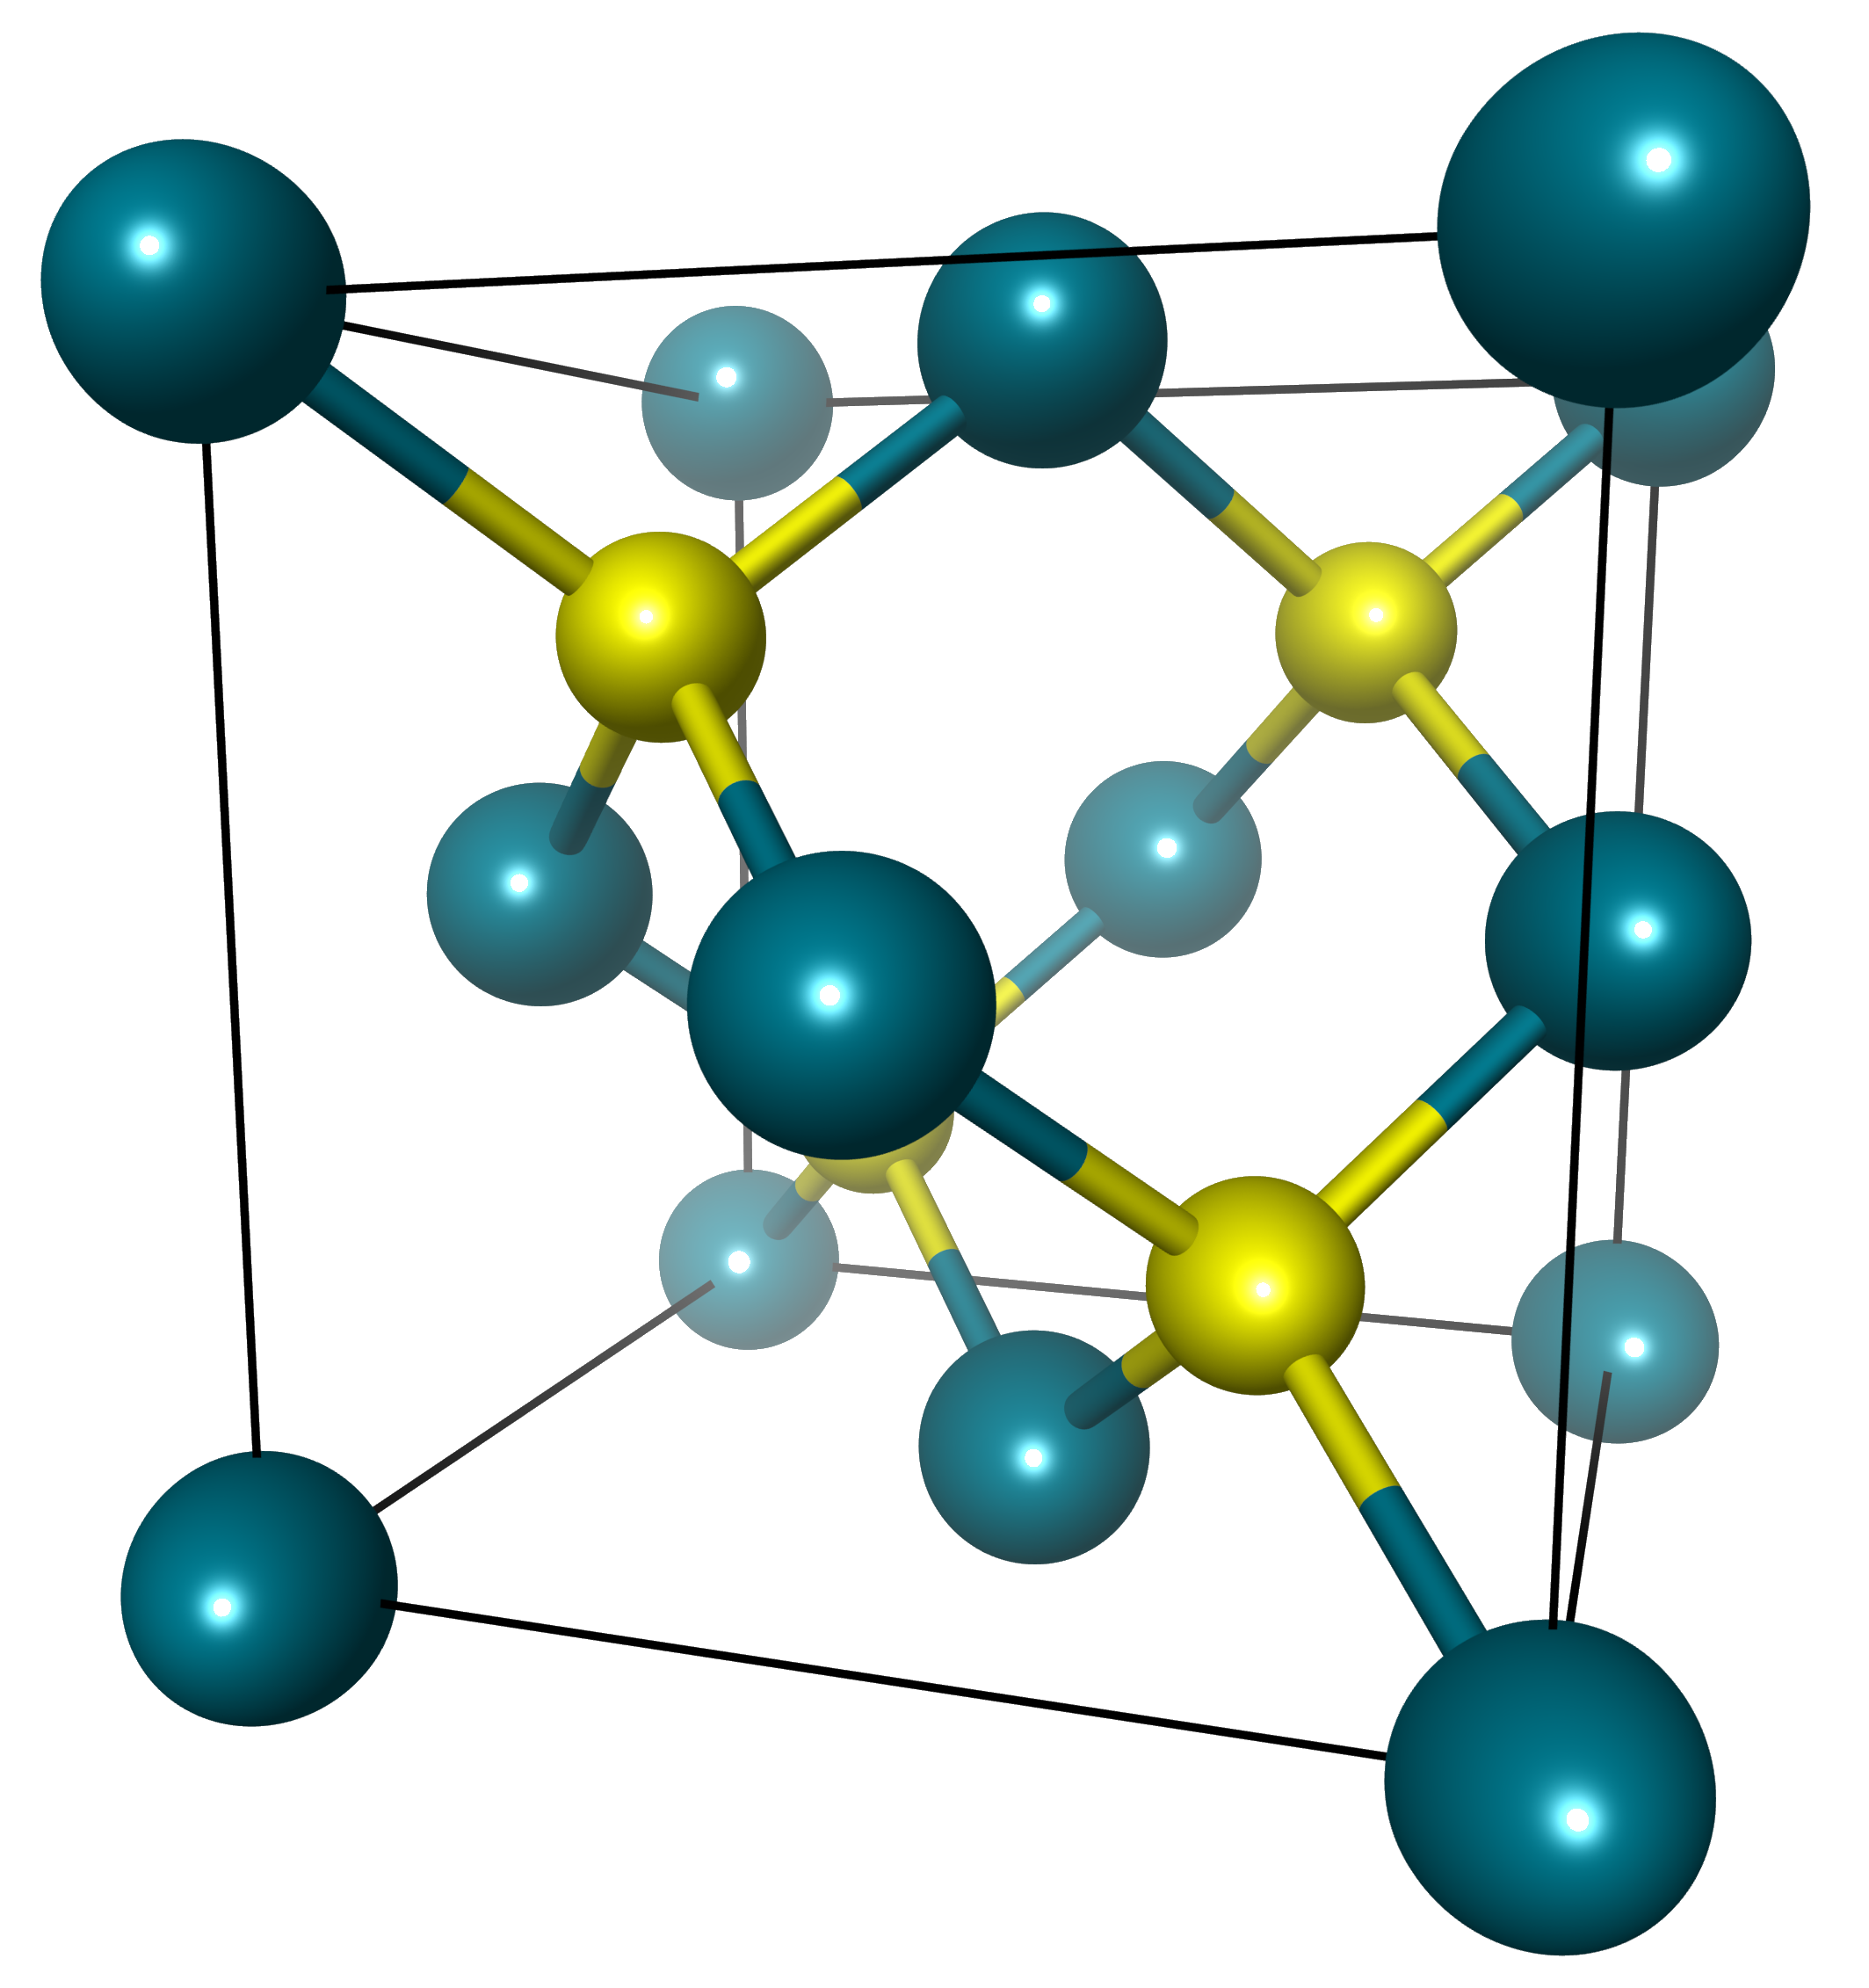
\includegraphics[width=0.3\textwidth]{../../../scripts/structures/GaAs-2}};
\node<3->[anchor=south east,text width=0.2\textwidth,font=\sffamily,xshift=-5mm,yshift=-8mm,scale=1.5,blue,inner sep=0mm](e1) at (s.south east){
\begin{equation*}
	\left(\tikzmarknode{a}{\mathcal{H}}-\varepsilon(\mathbf{k}\lambda)\ket{\mathbf{k\lambda}}\right)=0
\end{equation*}
};

\node<3->[anchor=south west,inner sep=0mm,yshift=0mm](bs) at (current page.south west){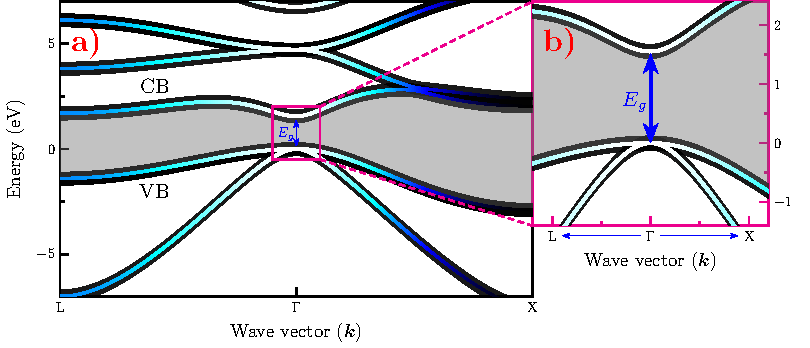
\includegraphics[width=1.05\textwidth]{../../figures/chapter-1/bands/build/bands01}};
\node<3->[anchor=south west,text width=0.6\textwidth,scale=1.1] at (bs.north west){Estructura de bandas para GaAs en bulto};
\end{tikzpicture}
\end{frame}
	
	
\subsection{Estructuras de baja dimensi\'on}
\begin{frame}[t]
	\frametitle{Introducci\'on}
	\framesubtitle{Estructuras de baja dimensi\'on}
	\vspace{-0.5cm}
	\begin{tikzpicture}[remember picture, overlay]
	\node<1->[anchor = north west, text width =0.75\textwidth, yshift = -0.75cm](txt) at (current page.north west) {
		\begin{tcolorbox}[enhanced,title =Estructuras de baja dimensi\'on,
		left=1mm,
		top=1mm,
		bottom=1mm,
		right=1mm,
		width =\textwidth,
		height=0.27\textheight,
		boxsep = 0cm,
		coltitle=blue,
		attach boxed title to top center={yshift=-2mm,yshifttext=-1mm},
		boxed title style={colframe=blue,
		colback=gc!70}]
		\begin{itemize}
		\item<1-> Semiconductor en bulto y su estructura de bandas
		\item<2-> Heteroestructuras semiconductoras 
		\item<3-> Heteroestructuras $\rightarrow$ Systemas nanoestructurados
		\item<4-> Primera approximaci\'on a los Pozos Cu\'anticos y su {\textcolor{magenta}{confinamiento}}
		\end{itemize}
		\end{tcolorbox}	
	};


	\node<1->[anchor=north east,xshift=-2cm,yshift=-1cm] at (current page.north east){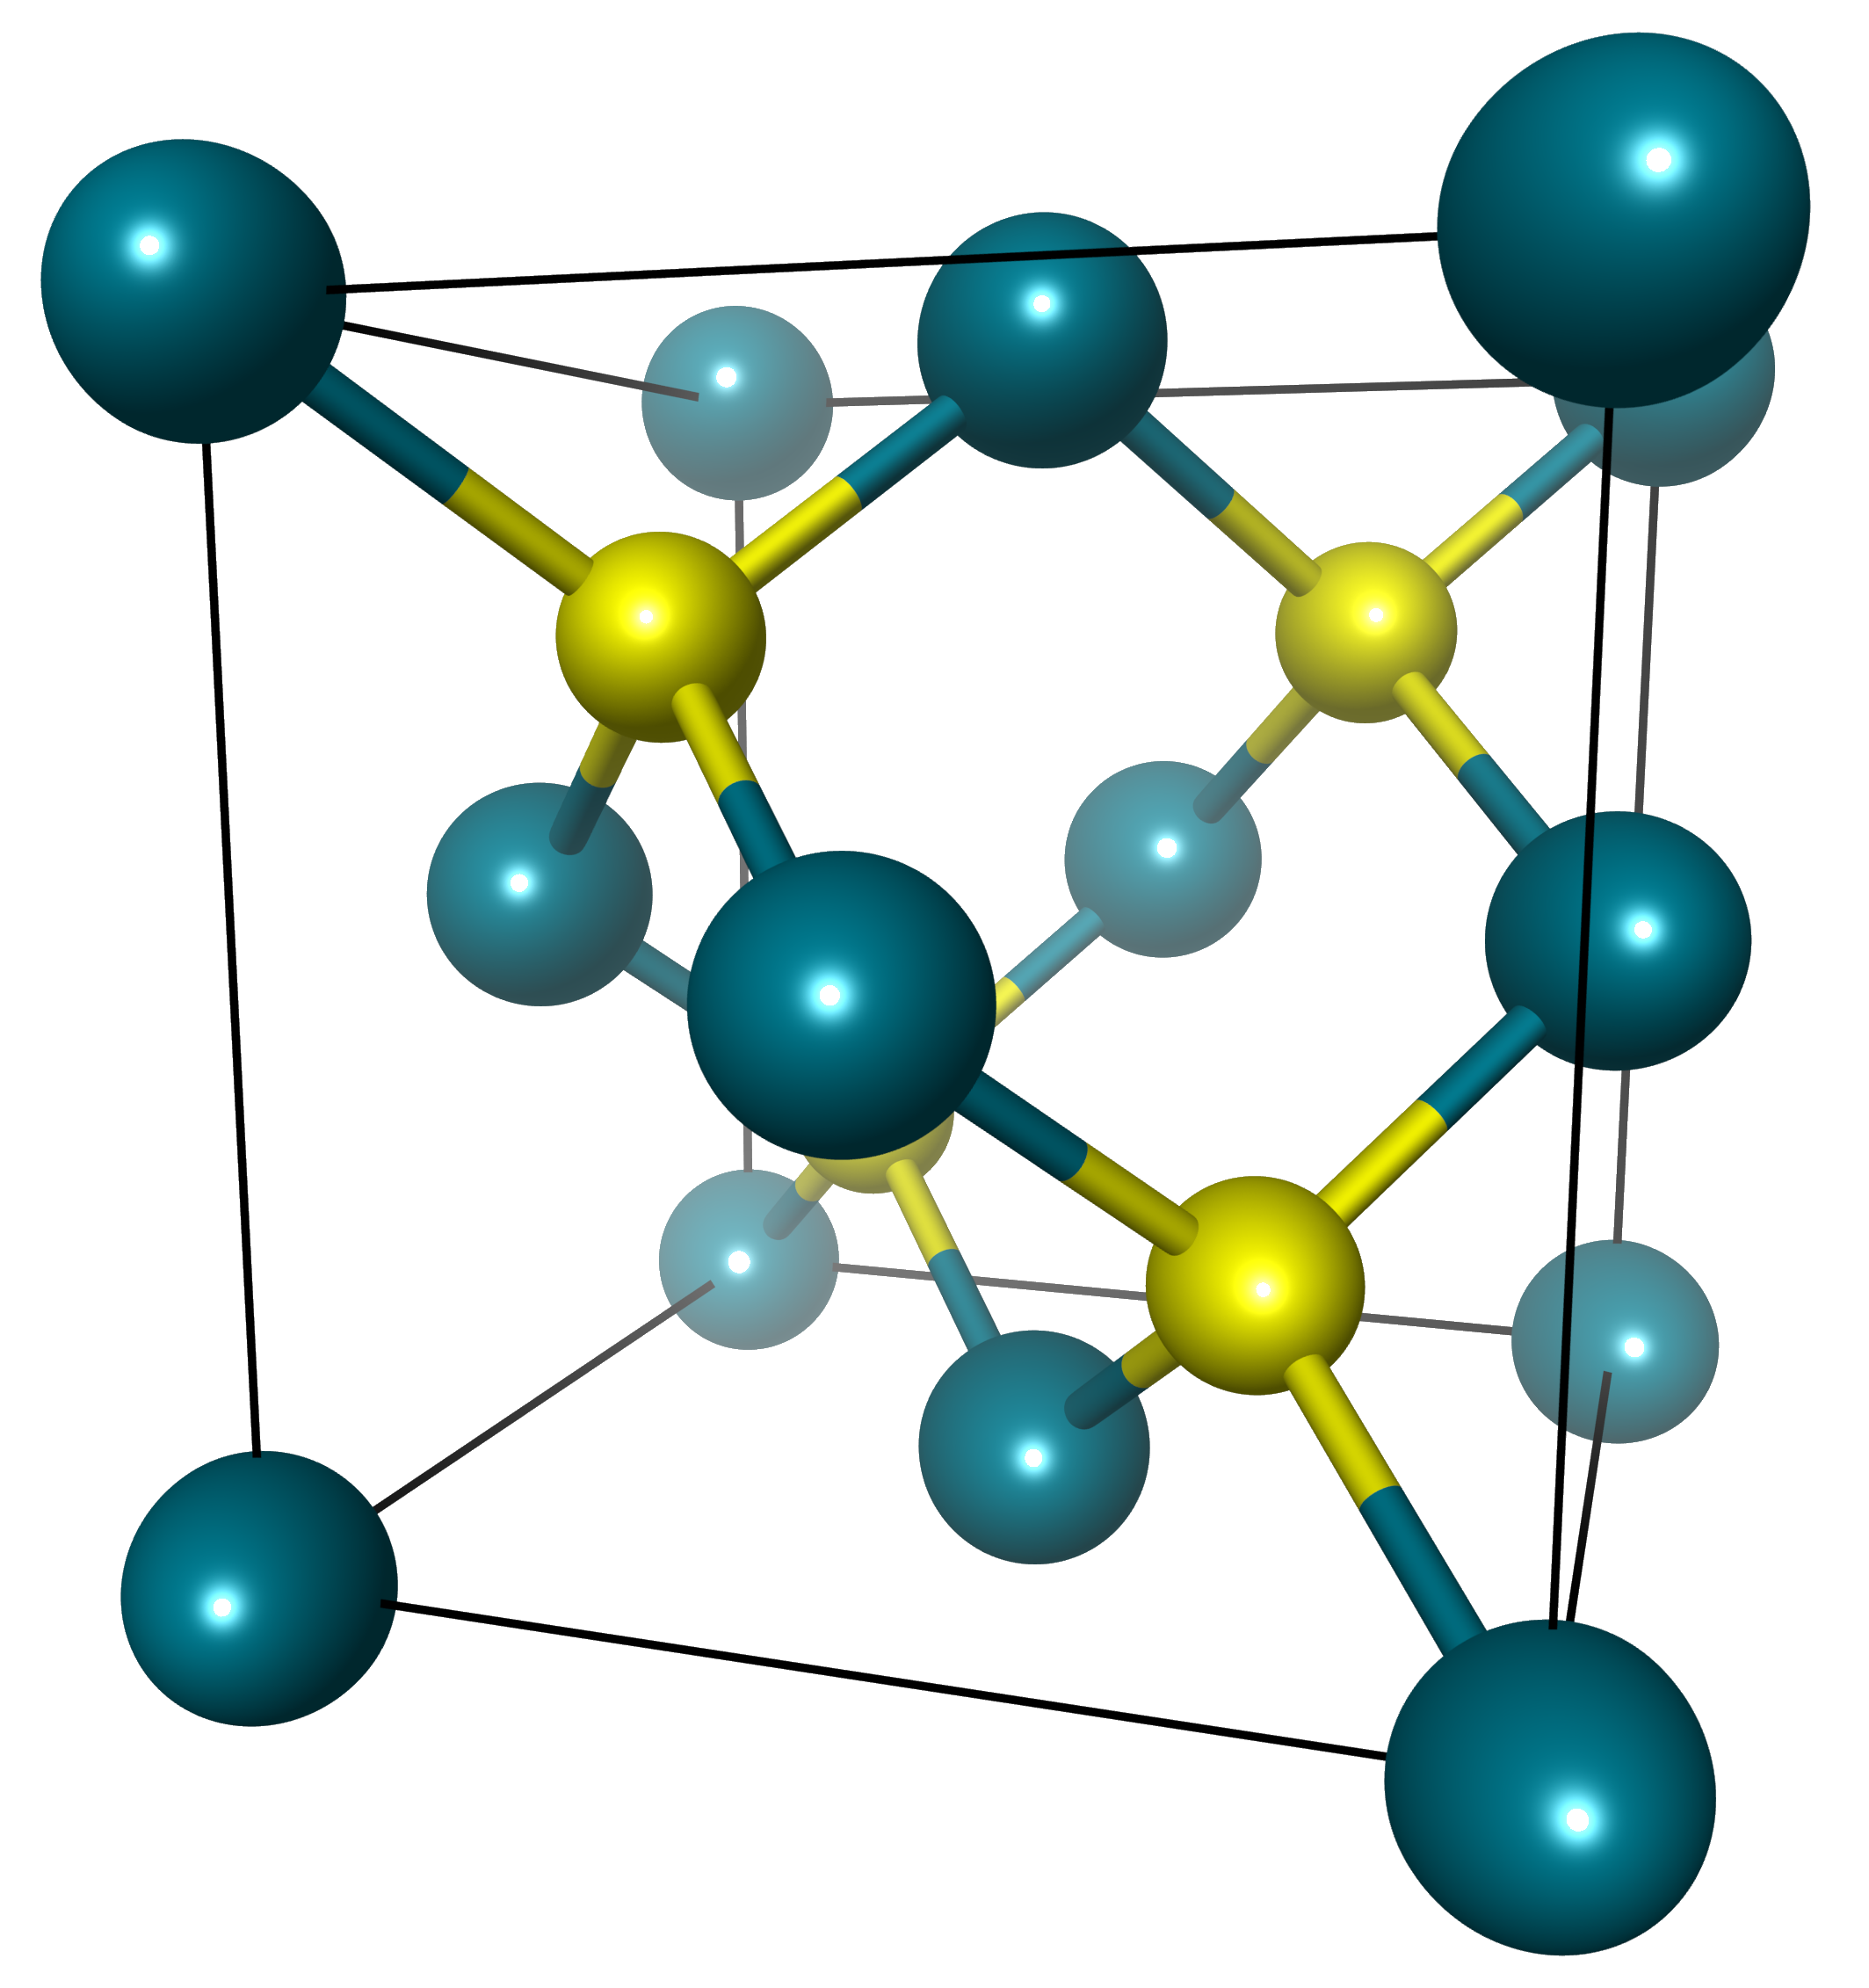
\includegraphics[width=0.25\textwidth]{../../../scripts/structures/GaAs-2}};
	\node<2>[anchor=south west,xshift=10mm] at (current page.south west){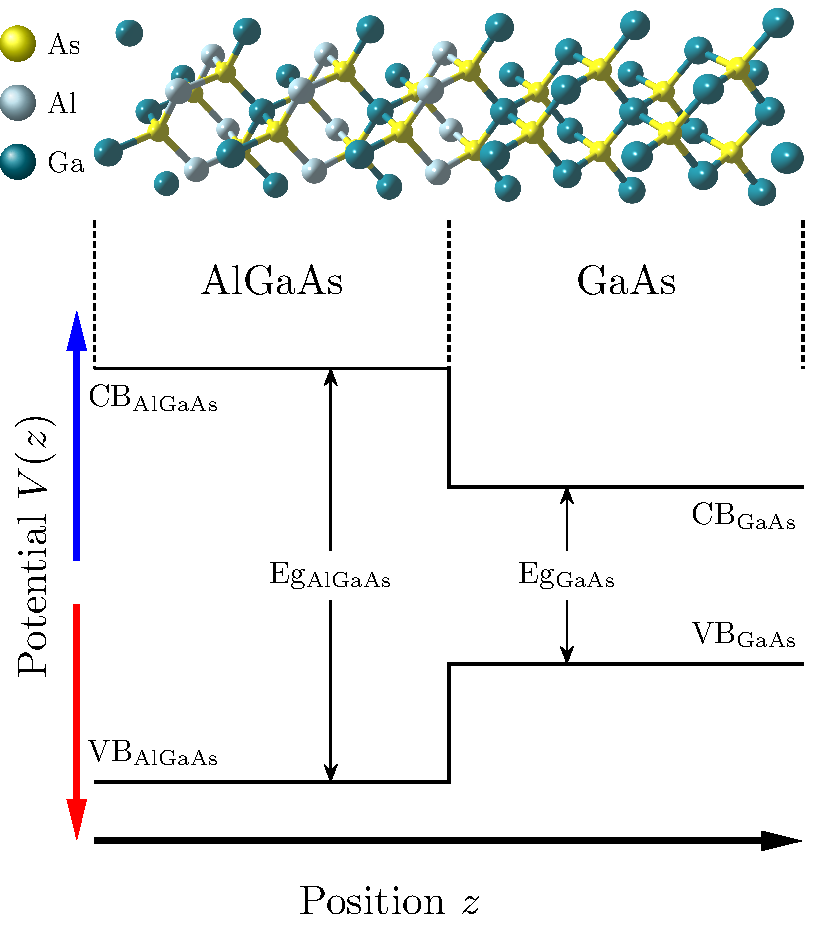
\includegraphics[width=0.59\textwidth]{../../figures/chapter-1/heterostructures/build-ruco/hs-01}};
	\node<3>[anchor=south west,xshift=10mm] at (current page.south west){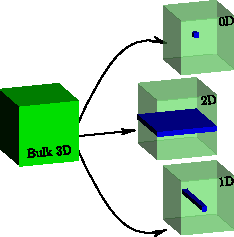
\includegraphics[width=0.59\textwidth]{../../figures/chapter-1/heterostructures/build-ruco/lds-00}};
	\node<4>[anchor=south west,xshift=0mm](qw1) at (current page.south west){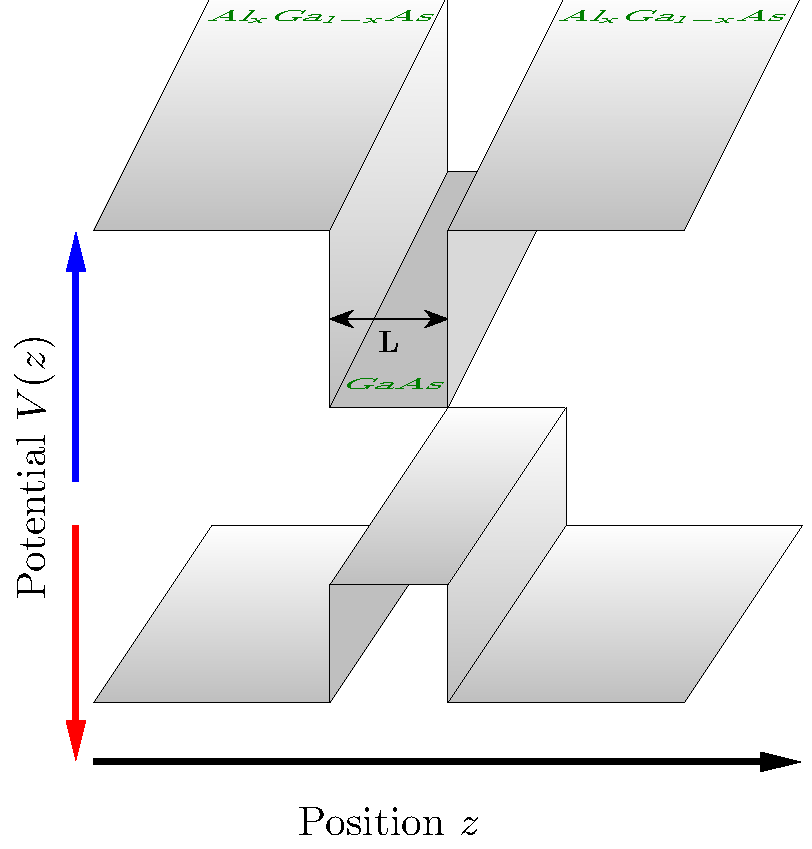
\includegraphics[width=0.48\textwidth]{../../figures/chapter-1/heterostructures/out/qw1}};
	\node<5>[anchor=south west,xshift=0mm](qw2) at (current page.south west){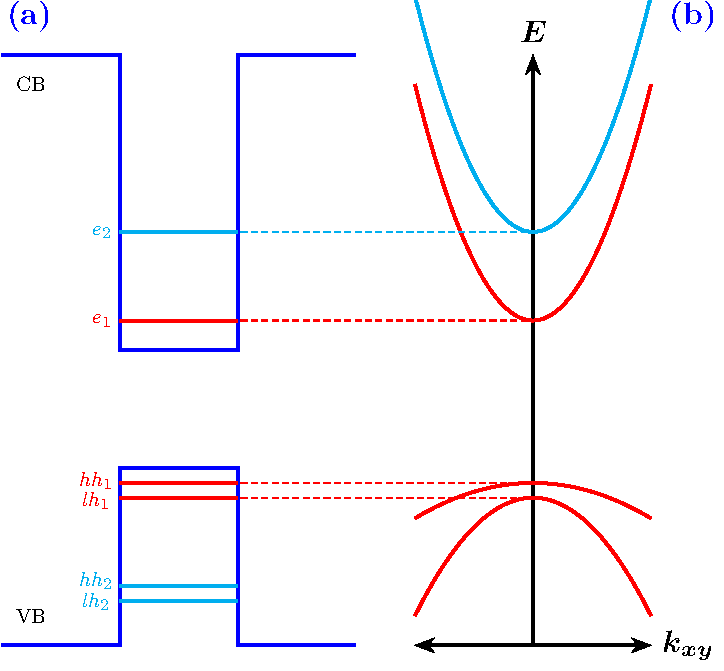
\includegraphics[width=0.55\textwidth]{../../figures/chapter-1/heterostructures/out/qw2}};

%equations
\node<4->[anchor=north west,xshift=5mm,blue](e1) at (qw1.north east){$-\dfrac{\hbar^{2}}{2m^{*}}\dfrac{\partial^{2}}{\partial {z}^{2}}\psi(z)+V(z)\psi(z)=E\psi(z)$};
\node<5->[anchor=north west,blue](e2) at (e1.south west){$E = E_{n} + \dfrac{\hbar^{2}|\boldsymbol{k}_{x,y}|^{2}}{2m^{*}}$};

\end{tikzpicture}
	\end{frame}
	